\documentclass[12pt]{article}

\usepackage[utf8]{inputenc}
\usepackage{latexsym,amsfonts,amssymb,amsthm,amsmath}
\usepackage{tikz}
\usepackage{stanli}
\usetikzlibrary{calc,through}
\usepackage{multicol}
\usepackage{geometry} 
\usepackage{enumitem}

\definecolor{darkred}{rgb}{0.6,0,0}

\setlength{\parindent}{0in}
\setlength{\oddsidemargin}{-0.25in}
\setlength{\textwidth}{7in}
\setlength{\textheight}{9.3in}
\setlength{\topmargin}{-1in}
\setlength{\headheight}{18pt}

\newcommand\blfootnote[1]{%
  \begingroup
  \renewcommand\thefootnote{}\footnote{#1}%
  \addtocounter{footnote}{-1}%
  \endgroup
}

\title{ME473 Dynamic Finite Element Analysis Mini-Project}
\author{Stefano Burzio}
\date{}

\begin{document}
\noindent ME473 - Dynamic finite element analysis of structures\hfill EPFL\\
Stefano Burzio \hfill 2025\\
\vspace{0.3cm}

\hspace*{\fill}\textbf{\Large Mini-project 3}\hspace*{\fill}
\begin{center}
  \textbf{\Large Modal and dynamic analysis of a mechanical \\[3pt] component or structure}
\end{center}

\hrulefill
\vspace{0.3cm}
\newline
{Project organization:}
\vspace{0.2cm}
\newline
\begin{minipage}[t]{0.38\textwidth}
  \begin{itemize}[itemsep=0.005cm]
    \item Individual project
    \item 20\% of final grade
    \item Pdf report: maximum 20 pages
  \end{itemize}
\end{minipage}
\hfill
\begin{minipage}[t]{0.58\textwidth}
  \begin{itemize}[itemsep=0.005cm]
    \item Programming language: \texttt{MATLAB}, \texttt{Abaqus}, \texttt{Ansys}
    \item Submission: January 9, 2026
    \item Total workload: 15h-20h
  \end{itemize}
\end{minipage}
\vspace{0.3cm}

\hrulefill

\begin{center}
  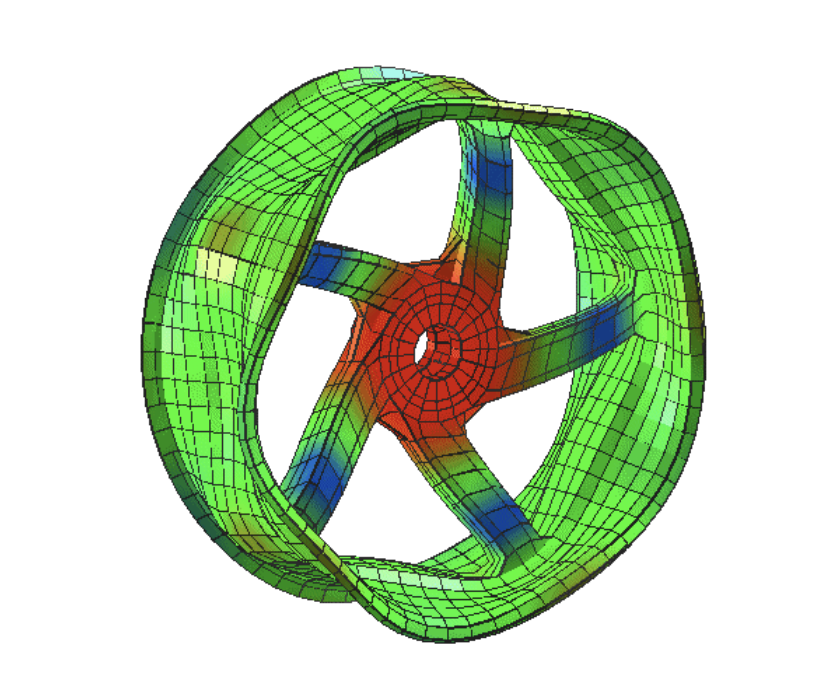
\includegraphics[width=0.5\textwidth]{../images/modalAnalysis.png}
\end{center}

\begin{enumerate}
  \item (Re)familiarize yourself with a well-known commercial finite element code such as Abaqus, Ansys or MATLAB PDE Toolbox.
  \item Choose one single mechanical component or structure requiring modal and time-domain dynamic analysis, describe the selected example, and justify the relevance of this choice. A connection to a current semester or master project is allowed.
  \item Model the chosen mechanical component or structure using solid and/or shell and/or beam finite elements to analyze its dynamic behavior, and discuss the mesh choice (type of finite elements, mesh density, convergence study, etc.).
  \item Determine the first five natural frequencies and mode shapes of the mechanical component or structure, and comment on the observed modal behavior.
  \item Choose a plausible excitation for the mechanical component or structure, describe and justify the chosen numerical method for time-domain solution, compute the time response to this excitation, and discuss the obtained results.
\end{enumerate}

\subsubsection*{Deliverables}
\begin{enumerate}
  \item \texttt{MATLAB}, \texttt{Abaqus}, \texttt{Ansys} files including:
        \begin{multicols}{2}
          \begin{itemize}
            \item Mesh definition
            \item Material and geometry properties
            \item Boundary conditions and loads
            \item Modal and dynamic analysis
          \end{itemize}
        \end{multicols}

  \item \textbf{PDF report:}
        \begin{enumerate}[label=\alph*.]
          \item Briefly describe the chosen mechanical component or structure, the motivation for its selection, and its relevance to a semester or master project if applicable.

          \item Explain the finite element modeling strategy, including:
                \begin{itemize}
                  \item Type of finite elements used (solid, shell, beam, etc.)
                  \item Mesh design, density, and any convergence studies performed
                  \item Material properties and geometric details
                  \item Boundary conditions and applied loads
                \end{itemize}

          \item Compute  the first five natural frequencies and corresponding mode shapes. Comment on the observed modal behavior and its physical significance.

          \item Describe the chosen excitation (e.g., force, displacement, or base motion), justify the selected time-domain solution method, and present the computed response over time. Discuss the results in terms of amplitude, resonance, and practical implications.

          \item Critically analyze the results, including potential sources of error, sensitivity to mesh refinement, and limitations of the model or numerical methods. Summarize the main findings of the modal and dynamic analysis and propose possible extensions or improvements for future studies.
        \end{enumerate}

  \item \textbf{Project defense:} prepare a PowerPoint, or similar, presentation of your project during the oral exam on January 14 (20 minutes presentation followed by a 10 minutes discussion). The presentation should:
        \begin{itemize}
          \item Summarize the project objectives, modeling approach, and chosen component/structure
          \item Highlight key results from the modal and dynamic analysis
          \item Include figures of mesh, mode shapes, and dynamic response
          \item Discuss conclusions and possible improvements
        \end{itemize}
\end{enumerate}

\end{document}